\documentclass[a4paper,12pt]{report}
\usepackage[utf8]{inputenc}
\usepackage[IL2]{fontenc}
\usepackage{listings}
\usepackage{amssymb}
\usepackage{amsmath}
\usepackage{url}
\usepackage{graphicx}
\usepackage[czech]{babel}
\begin{document}
\chapter{Praktická část}
  V této kapitole se budeme věnovat praktické aplikaci Markowitzovy teorie potrfolia. Jako nástroj ke zpracování dat poslouží rozšířený a několika chyb zbavený skript Travise Vaughta\cite{tvaught}. Je napsán v jazyce Python a využívá knihoven NumPy. Zdrojový kód původní verze je dostupný na internetu\cite{source}.
  
  Software je založen na Markowitzově teorii a k analýze aktiv historickou metodou používa metrik z CAPM. Samotný výpočet optima probíhá numerickou iterativní metodou převzatou z práce Williama Sharpa\cite{sharpe}.
  
  Zdrojem dat je Yahoo! Finance\cite{yahoo}. Byly použity výhradně akcie z indexu S\&P500, protože obsahuje známé a stabilní společnosti, do kterých je zároveň snadné investovat. Historický obdobím pro získání metrik je 1.1.2010 až 1.11.2011. Jako tolerance k risku pro finální optimalizaci byla zvolena poměrně nízká hodnota 0,05 ročně, která zajistí vyšší pestrost portfolia. Bezrizikové aktivum má nulový výnos a není povoleno obchodování na krátko.
  \section{Hardware}
    Toto portfolio obsahuje významné výrobce počítačového hardware. Z tabulek je patrno, že největšího ročního výnosu dosahuje Apple Inc. a nejnižšího rizika IBM, přičemž si stále zachovává slušný růst. Optimalizované portfolio obsahuje právě tyto dvě akcie a dále ještě nepatrný podíl Intel Corporation. Jeho volatilita je 0.193, což je méně než obě hlavní akcie. Roční výnos dosahuje 24.37\%, tedy více než má samostatně nejméně riziková akcie.
    \begin{table}[htb]
      \centering
      \begin{tabular}{|l|l|r|r|}
        \hline
        Symbol&Název&Volatilita&Roční výnos\\\hline\hline
        A&Agilent Technologies &0.402&16.43\%\\\hline
        AAPL&Apple Inc. &0.266&37.57\%\\\hline
        AMD&Advanced Micro Devices &0.497&-16.46\%\\\hline
        DELL&Dell Inc. &0.345&9.585\%\\\hline
        HPQ&Hewlett-Packard &0.334&-31.4\%\\\hline
        IBM&International Bus. Machines &0.198&20.96\%\\\hline
        INTC&Intel Corp. &0.254&14.2\%\\\hline
        NVDA&Nvidia Corporation &0.512&-0.09651\%\\\hline
        TXN&Texas Instruments &0.267&13.72\%\\\hline
      \end{tabular}
      \caption{Akcie pro porfolio hardware}
    \end{table}

    \begin{figure}[htb]
      \centering
        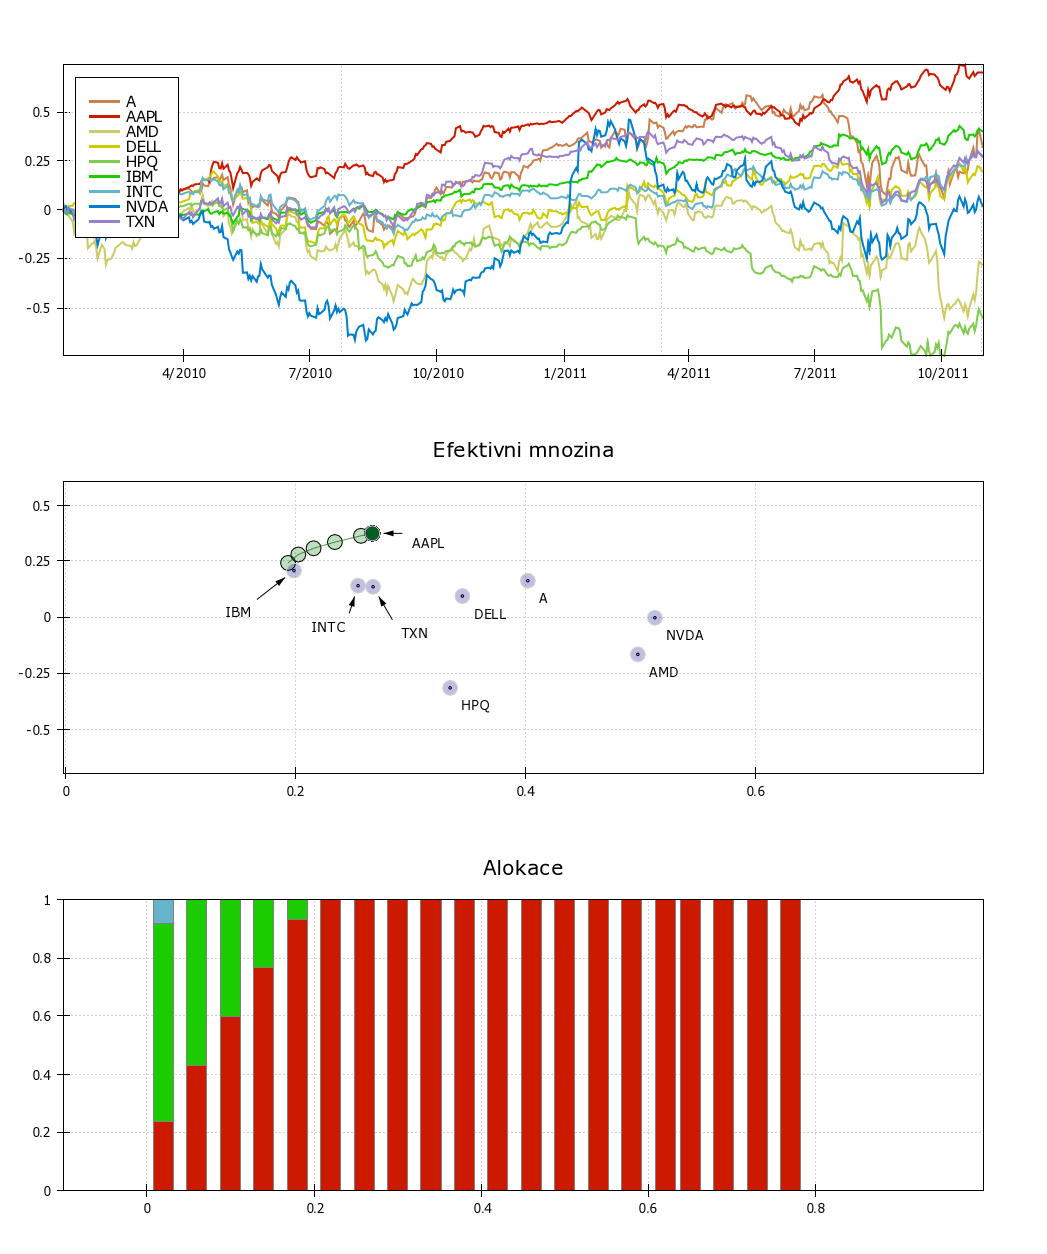
\includegraphics[height=0.95\textheight]{hw1.png}
       \caption{Grafické zobrazení portfolia hardware}
    \end{figure}

    \begin{table}[htb]
      \centering
      \begin{tabular}{|l|l|r|}
        \hline
        Symbol&Název&Alokace\\\hline\hline
        AAPL&Apple Inc. &0.346\\\hline
        IBM&International Bus. Machines &0.648\\\hline
        INTC&Intel Corp. &0.0069\\\hline
      \end{tabular}
      \caption{Optimální portfolio hardware}
    \end{table}
    
  \clearpage
  \section{Software a internetové služby}
    Zde se zabýváme velkými softwarovými firmami a poskytovateli elektronických služeb. Z metrik je vidět, že tyto akcie dosahují nemalých zhodnocení, ovšem často za cenu vysoké volatility. Optimalizované portfolio má nízký roční výnos 3,736\% a poměrně vysokou volatilitu 0.218, která je ovšem menší než u jakékoliv jednotlivé akcie ze sektoru. Je to způsobeno tím, že akcie firmy Microsoft má záporný roční výnos -4.513\%, ale přesto tvoří více než polovinu potfolia, neboť je vnímána jako konkurent k v podstatě všem ostatním, což způsobuje silnou zápornou korelaci. 
    \begin{table}[htb]
      \centering
      \begin{tabular}{|l|l|r|r|}
        \hline
        Symbol&Název&Volatilita&Roční výnos\\\hline\hline
        ADBE&Adobe Systems &0.356&-7.255\%\\\hline
        ADSK&Autodesk Inc. &0.397&23.36\%\\\hline
        AKAM&Akamai Technologies Inc &0.478&12.77\%\\\hline
        EBAY&eBay Inc. &0.35&20.87\%\\\hline
        ERTS&Electronic Arts &0.362&19.38\%\\\hline
        GOOG&Google Inc. &0.291&0.1524\%\\\hline
        MSFT&Microsoft Corp. &0.226&-4.513\%\\\hline
        ORCL&Oracle Corp. &0.287&19.16\%\\\hline
        SYMC&Symantec Corp. &0.306&-0.5626\%\\\hline
        YHOO&Yahoo Inc. &0.351&0.2939\%\\\hline
      \end{tabular}
      \caption{Akcie pro porfolio software}
    \end{table}

    \begin{figure}[htb]
      \centering
        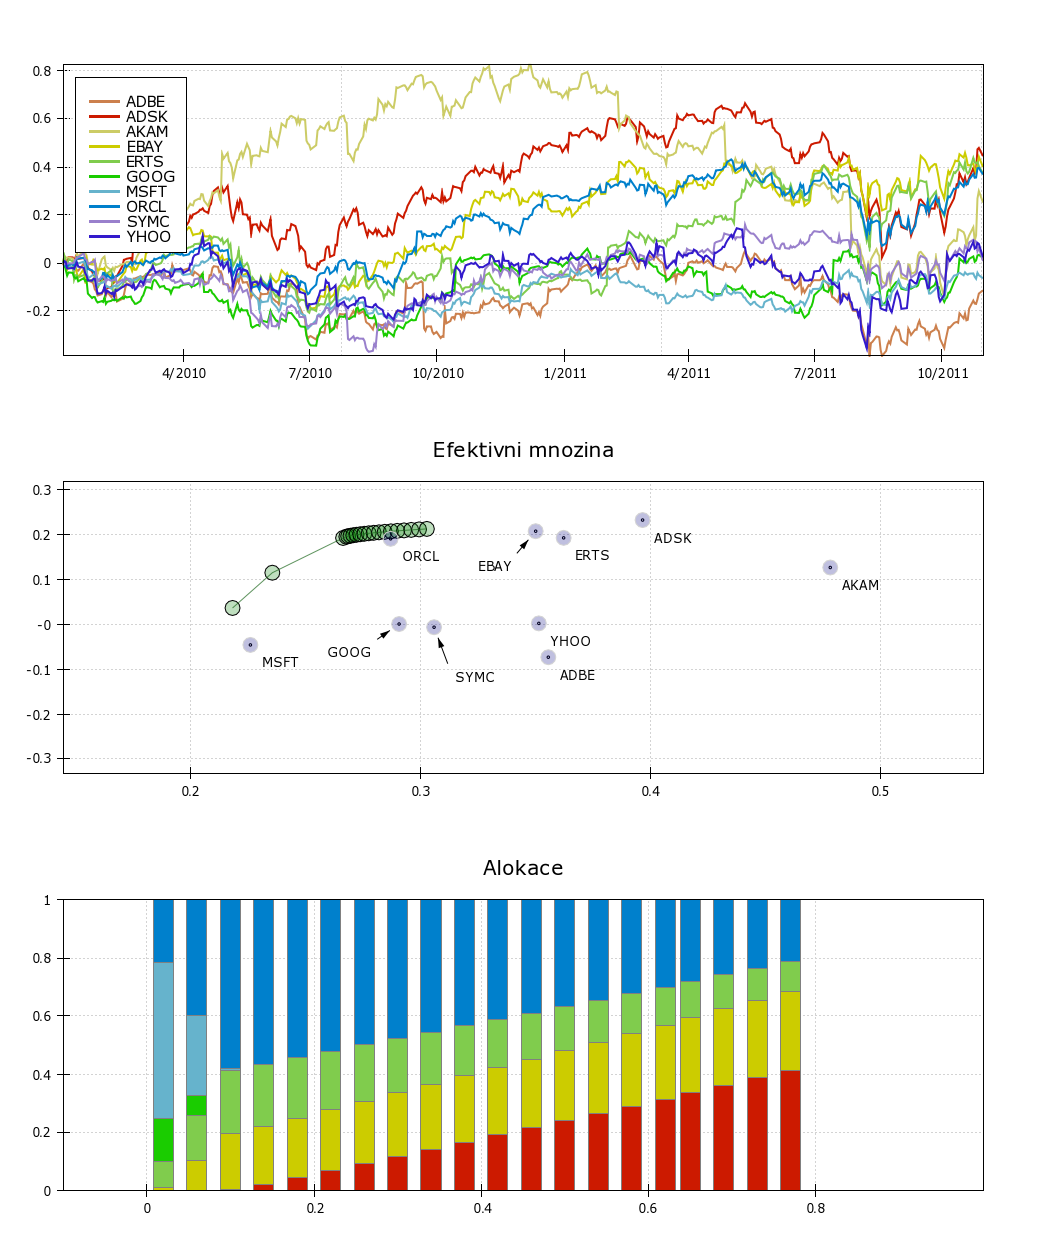
\includegraphics[height=0.95\textheight]{sw1.png}
       \caption{Grafické zobrazení portfolia software}
    \end{figure}

    \begin{table}[htb]
      \centering
      \begin{tabular}{|l|l|r|}
        \hline
        Symbol&Název&Alokace\\\hline\hline
        EBAY&eBay Inc. &0.0129\\\hline
        ERTS&Electronic Arts &0.0888\\\hline
        GOOG&Google Inc. &0.149\\\hline
        MSFT&Microsoft Corp. &0.534\\\hline
        ORCL&Oracle Corp. &0.216\\\hline
      \end{tabular}
      \caption{Optimální portfolio software}
    \end{table}

  \clearpage
  \section{Výrobci farmaceutik}
    Dalším sektorem jsou výrobci farmaceutik. Z tabulek ihned vidíme, že všechny akcie mají v podstatě stejný charakter -- nízký výnos i volatilitu. Přesto se optimalizací podařilo dosáhnout volatility 0.137, což je méně než má kterákoliv akcie. Výnos 3.359\% je přibližně aritmetický průměr výnosů v sektoru.
    
    \begin{table}[htb]
      \centering
      \begin{tabular}{|l|l|r|r|}
        \hline
        Symbol&Název&Volatilita&Roční výnos\\\hline\hline
        ABT&Abbott Labs &0.16&3.525\%\\\hline
        BAX&Baxter International Inc. &0.244&1.14\%\\\hline
        JNJ&Johnson \& Johnson &0.15&3.236\%\\\hline
        MRK&Merck \& Co. &0.213&1.664\%\\\hline
        PFE&Pfizer Inc. &0.226&6.494\%\\\hline
      \end{tabular}
      \caption{Akcie pro porfolio farmaceutik}
    \end{table}

    \begin{figure}[htb]
      \centering
        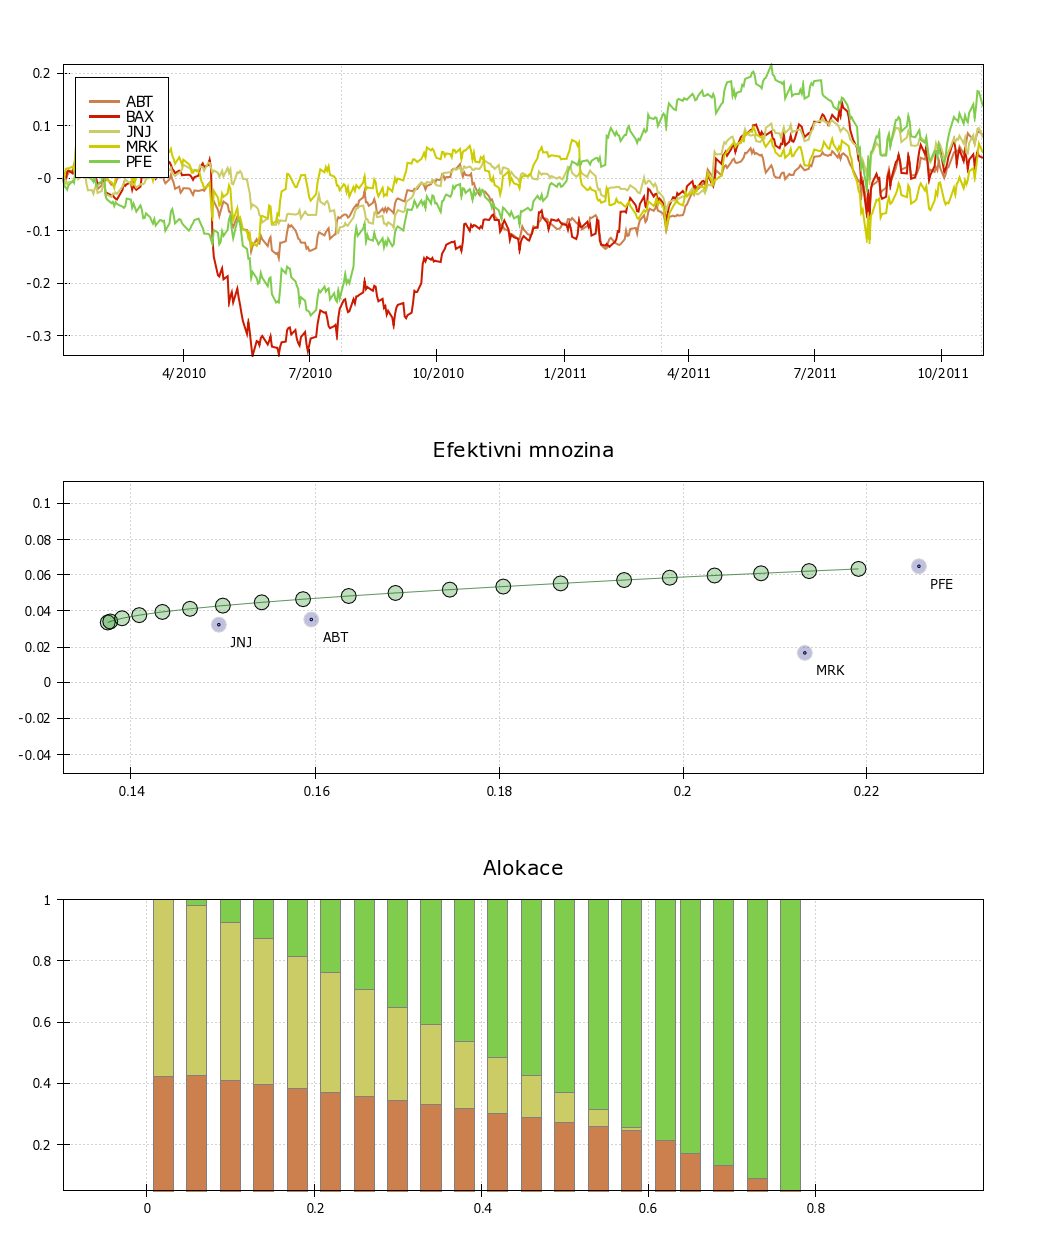
\includegraphics[height=0.95\textheight]{drugs1.png}
       \caption{Grafické zobrazení portfolia farmaceutik}
    \end{figure}

    \begin{table}[htb]
      \centering
      \begin{tabular}{|l|l|r|}
        \hline
        Symbol&Název&Alokace\\\hline\hline
        ABT&Abbott Labs &0.424\\\hline
        JNJ&Johnson \& Johnson &0.576\\\hline
      \end{tabular}
      \caption{Optimální portfolio farmaceutik}
    \end{table}
    
  \clearpage
  \section{Finanční sektor}
    Sektor financí obsahuje velmi rozličné akciové tituly. Výnosy se pohybují od -34\% do +17\%. Společná je však velmi vysoká volatilita. Optimalizací se ji podřilo dramaticky snížít na 0.286 při zachování přijatelného výnosu 9.456\%. Zde akcie Goldman Sachs působí přes výraznou ztrátu jako stabilizátor.
    
    \begin{table}[htb]
      \centering
      \begin{tabular}{|l|l|r|r|}
        \hline
        Symbol&Název&Volatilita&Roční výnos\\\hline\hline
        AXP&American Express &0.315&17.55\%\\\hline
        BAC&Bank of America Corp. &0.479&-34.62\%\\\hline
        C&Citigroup Inc. &0.445&5.03\%\\\hline
        GS&Goldman Sachs Group &0.331&-19.59\%\\\hline
        JPM&JPMorgan Chase \& Co. &0.343&-5.188\%\\\hline
        MS&Morgan Stanley &0.457&-20.4\%\\\hline
        NDAQ&NASDAQ OMX Group &0.352&16.9\%\\\hline
        NYX&NYSE Euronext &0.398&12.58\%\\\hline
      \end{tabular}
      \caption{Akcie pro porfolio financí}
    \end{table}

    \begin{figure}[htb]
      \centering
        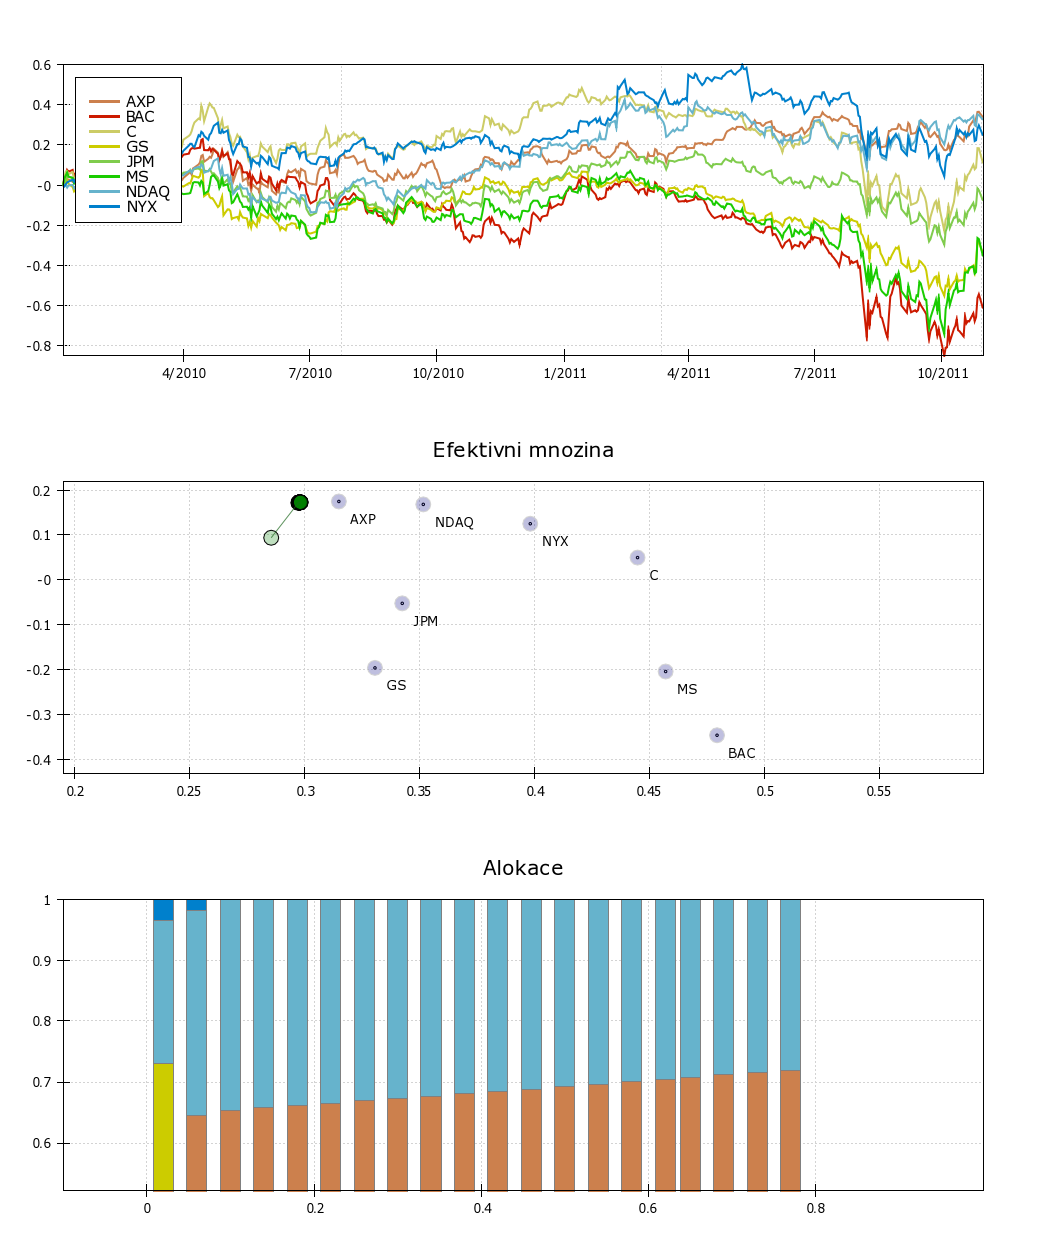
\includegraphics[height=0.95\textheight]{fin1.png}
       \caption{Grafické zobrazení portfolia financí}
    \end{figure}

    \begin{table}[htb]
      \centering
      \begin{tabular}{|l|l|r|}
        \hline
        Symbol&Název&Alokace\\\hline\hline
        AXP&American Express &0.522\\\hline
        GS&Goldman Sachs Group &0.209\\\hline
        NDAQ&NASDAQ OMX Group &0.235\\\hline
        NYX&NYSE Euronext &0.0341\\\hline
      \end{tabular}
      \caption{Optimální portfolio financí}
    \end{table}
    
  \clearpage
  \section{Průmysl}
    V sektoru průmyslu vidíme až na společnost 3M solidní výnosnost za přiměřené volatility. Caterpillar dosahuje ročního zhodnocení dokonce přes 33\%. V našem optimalizovaném nízkorizikové portfoliu se přesto neobjevuje, protože je příliš silně pozitivně korelován s ostatními. Dosahujeme nižšího výnosu 6.073\% a stejně tak volatility 0.236 z toho důvodu, že přes 60\%  portfolio tovří 3M.
    
    \begin{table}[htb]
      \centering
      \begin{tabular}{|l|l|r|r|}
        \hline
        Symbol&Název&Volatilita&Roční výnos\\\hline\hline
        BA&Boeing Company &0.299&14.5\%\\\hline
        CAT&Caterpillar Inc. &0.34&33.5\%\\\hline
        GE&General Electric &0.286&10.3\%\\\hline
        HON&Honeywell Int'l Inc. &0.29&20.14\%\\\hline
        MMM&3M Company &0.24&1.624\%\\\hline
      \end{tabular}
      \caption{Akcie pro porfolio průmyslu}
    \end{table}

    \begin{figure}[htb]
      \centering
        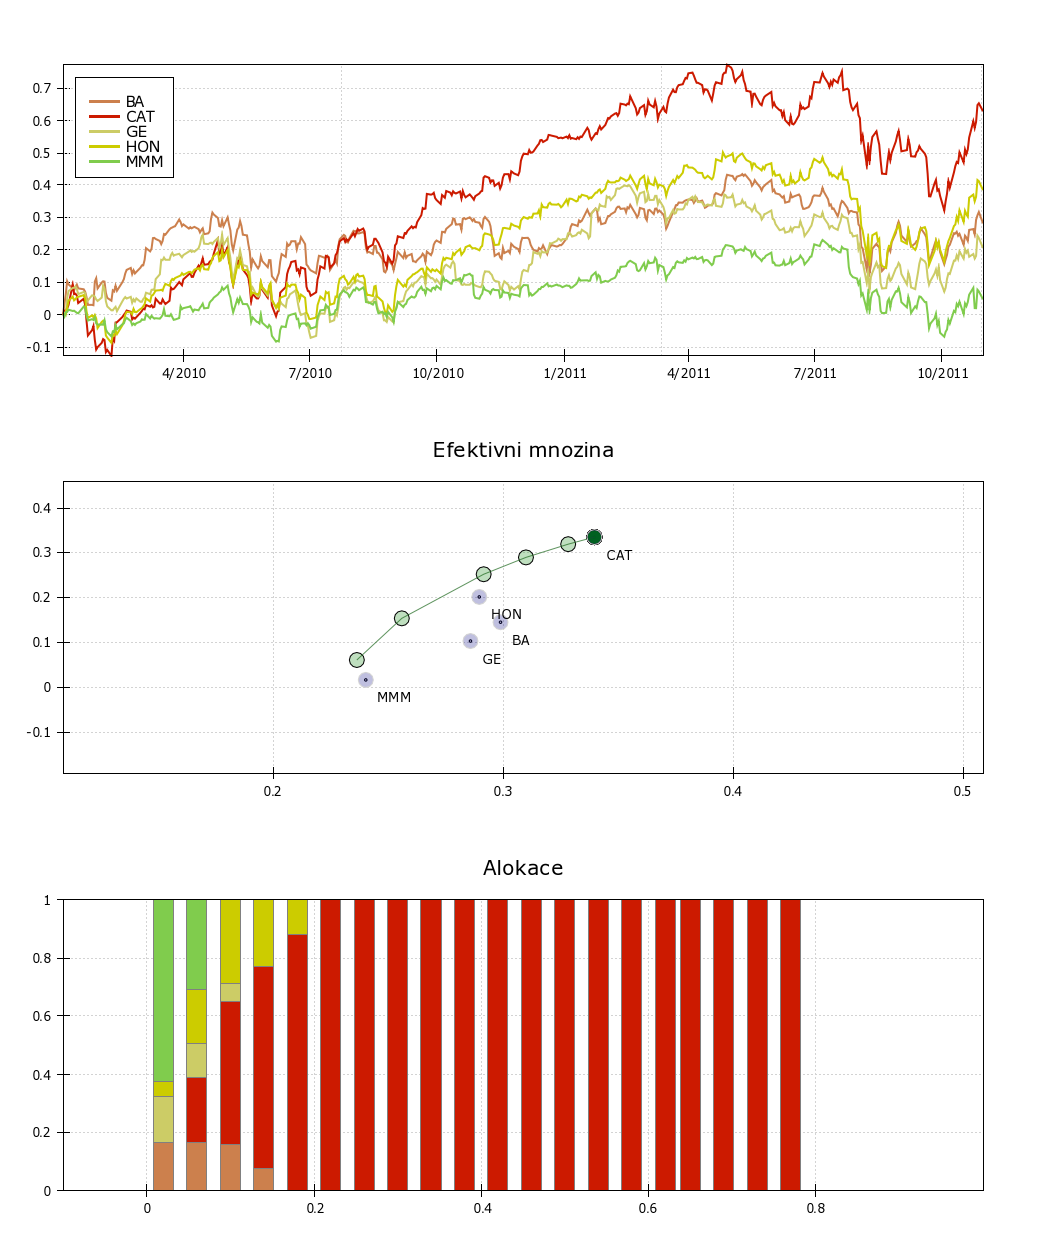
\includegraphics[height=0.95\textheight]{ind1.png}
       \caption{Grafické zobrazení portfolia průmyslu}
    \end{figure}

    \begin{table}[htb]
      \centering
      \begin{tabular}{|l|l|r|}
        \hline
        Symbol&Název&Alokace\\\hline\hline
        BA&Boeing Company &0.165\\\hline
        GE&General Electric &0.16\\\hline
        HON&Honeywell Int'l Inc. &0.0501\\\hline
        MMM&3M Company &0.624\\\hline
      \end{tabular}
      \caption{Optimální portfolio průmyslu}
    \end{table}
    
  \clearpage
  \section{Nejcennější značky}
    Zde budeme zkoumat akcie majitelů 10 nejcennějších značek podle Financial Times\cite{ft}, které jsou obsaženy v S\&P500. Snad až na Altria Group, která je majitelem značky Marlboro, jsou všechny jasné. Jsou zde obsaženy tituly sektorů IT, komunikací, průmyslu i konzumního zboží. Díky této diverzitě bylo dosaženo nízké volatility 0.136 a vysokého výnosu 24.24\%.   
    \begin{table}[htb]
      \centering
      \begin{tabular}{|l|l|r|r|}
        \hline
        Symbol&Název&Volatilita&Roční výnos\\\hline\hline
        AAPL&Apple Inc. &0.266&37.57\%\\\hline
        GE&General Electric &0.286&10.3\%\\\hline
        GOOG&Google Inc. &0.291&0.1524\%\\\hline
        IBM&International Bus. Machines &0.198&20.96\%\\\hline
        KO&Coca Cola Co. &0.164&13.13\%\\\hline
        MCD&McDonald's Corp. &0.161&24.78\%\\\hline
        MO&Altria Group Inc. &0.157&24.47\%\\\hline
        MSFT&Microsoft Corp. &0.226&-4.513\%\\\hline
        T&AT\&T Inc. &0.166&8.371\%\\\hline
        VZ&Verizon Communications &0.18&12.74\%\\\hline
      \end{tabular}
      \caption{Akcie pro porfolio značek}
    \end{table}

    \begin{figure}[htb]
      \centering
        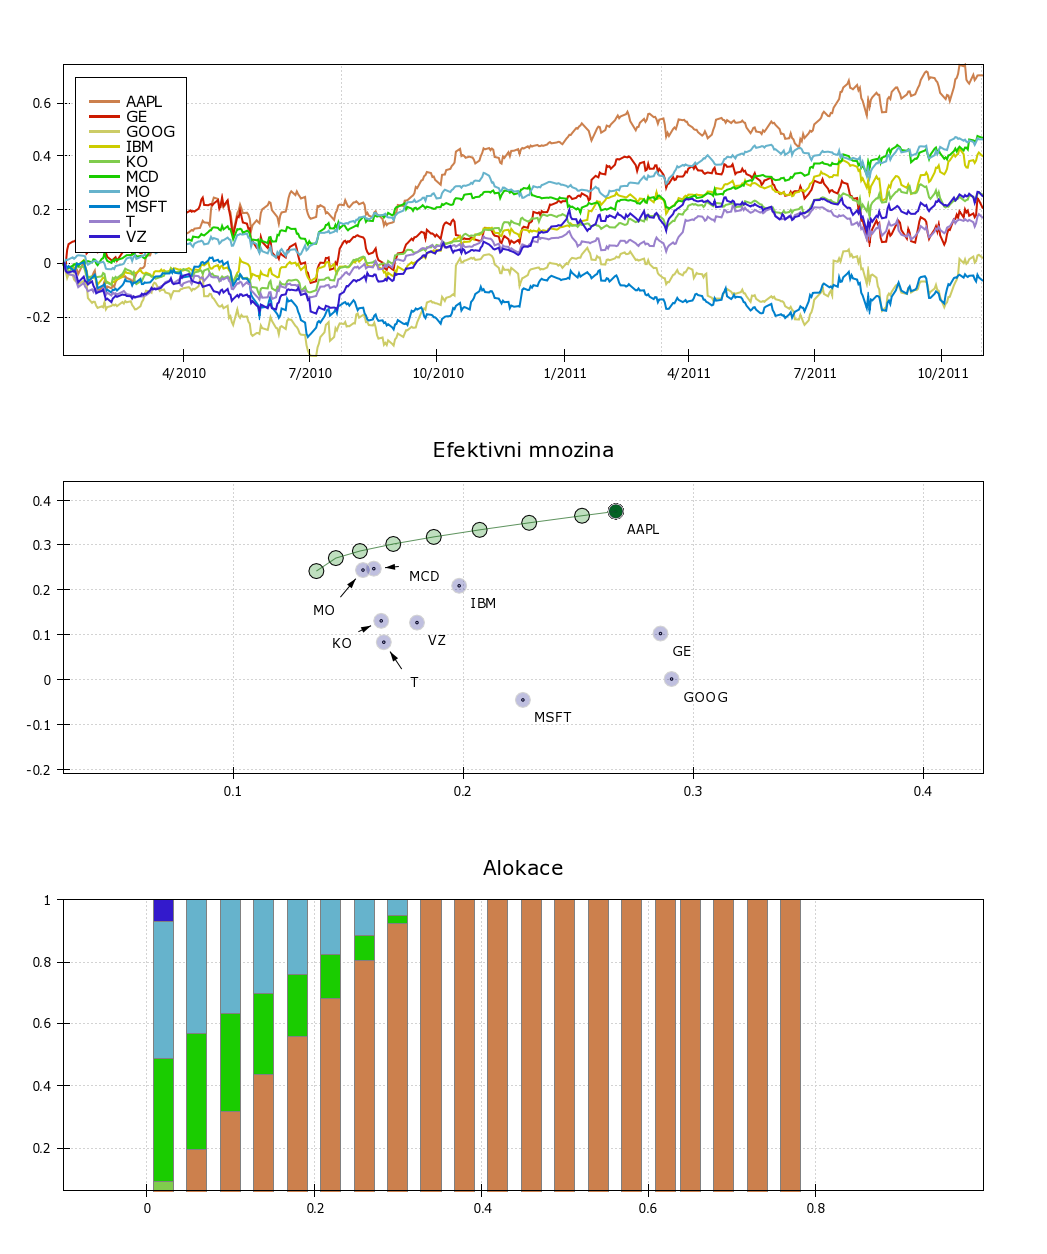
\includegraphics[height=0.95\textheight]{brands1.png}
       \caption{Grafické zobrazení portfolia značek}
    \end{figure}

    \begin{table}[htb]
      \centering
      \begin{tabular}{|l|l|r|}
        \hline
        Symbol&Název&Alokace\\\hline\hline
        AAPL&Apple Inc. &0.0617\\\hline
        KO&Coca Cola Co. &0.0311\\\hline
        MCD&McDonald's Corp. &0.394\\\hline
        MO&Altria Group Inc. &0.444\\\hline
        VZ&Verizon Communications &0.0688\\\hline
      \end{tabular}
      \caption{Optimální portfolio značek}
    \end{table}
    
  \clearpage
  \section{Deset nejziskovějších titulů}
    Tento seznam nejziskovějších titulů byl získán výpočtem příslušných metrik pro všechny akcie S\&P500. Opět vidíme společnosti ze všech oblastí hospodářství. Optimalizací bylo získáno portfolio s volatilitou 0.214 a vysokým výnosem 46.52\%, na který se ovšem vzhledem k použití čistě historické metody nelze do budoucna spolehnout.
    \begin{table}[htb]
      \centering
      \begin{tabular}{|l|l|r|r|}
        \hline
        Symbol&Název&Volatilita&Roční výnos\\\hline\hline
        ACAS&American Capital Strategies Ltd &0.502&72.66\%\\\hline
        AN&AutoNation Inc. &0.352&43.83\%\\\hline
        ANF&Abercrombie \& Fitch Co. &0.457&52.22\%\\\hline
        BIIB&BIOGEN IDEC Inc. &0.303&46.06\%\\\hline
        CMI&Cummins Inc. &0.417&50.12\%\\\hline
        EL&Estee Lauder Cos. &0.317&43.38\%\\\hline
        EP&El Paso Corp. &0.39&55.31\%\\\hline
        FDO&Family Dollar Stores &0.302&46.62\%\\\hline
        LTD&Limited Brands Inc. &0.346&50.85\%\\\hline
        MBI&MBIA Inc. &0.644&60.09\%\\\hline
      \end{tabular}
      \caption{Akcie pro porfolio Top10}
    \end{table}

    \begin{figure}[htb]
      \centering
        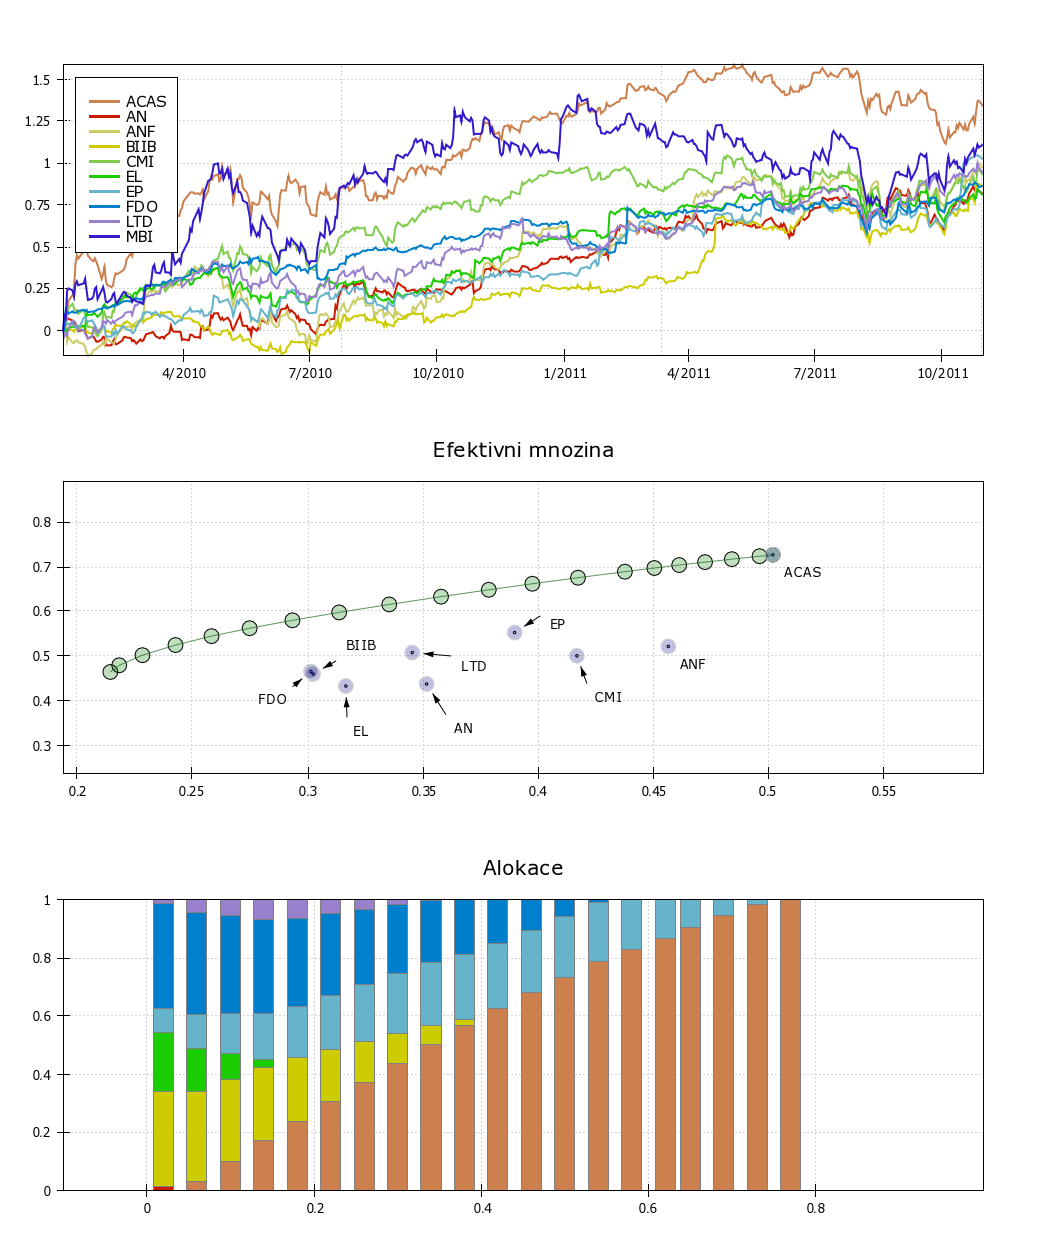
\includegraphics[height=0.95\textheight]{top10.png}
       \caption{Grafické zobrazení portfolia Top10}
    \end{figure}

    \begin{table}[htb]
      \centering
      \begin{tabular}{|l|l|r|}
        \hline
        Symbol&Název&Alokace\\\hline\hline
        AN&AutoNation Inc. &0.0163\\\hline
        BIIB&BIOGEN IDEC Inc. &0.326\\\hline
        EL&Estee Lauder Cos. &0.201\\\hline
        EP&El Paso Corp. &0.0828\\\hline
        FDO&Family Dollar Stores &0.36\\\hline
        LTD&Limited Brands Inc. &0.014\\\hline

      \end{tabular}
      \caption{Optimální portfolio Top10}
    \end{table}

  \clearpage
  \section{Celý S\&P500}
    Zde byl algoritmus spuštěn na všechny akcie z S\&P500, které nevykazovaly při zpracování chybu. Výsledkem je následující portfolio s volatilitou 0.119 a výnosem 30.32\%.

    \begin{table}[htb]
      \centering
      \begin{tabular}{|l|l|r|r|r|}
        \hline
        Symbol&Název&Alokace&Volatilita&Roční výnos\\\hline\hline
        AZO&AutoZone Inc. &0.287&0.177&39.94\%\\\hline
        BIIB&BIOGEN IDEC Inc. &0.0446&0.303&46.06\%\\\hline
        FDO&Family Dollar Stores &0.0744&0.302&46.62\%\\\hline
        HSY&The Hershey Company &0.127&0.198&28.72\%\\\hline
        MCD&McDonald's Corp. &0.0317&0.161&24.78\%\\\hline
        MO&Altria Group Inc. &0.105&0.157&24.47\%\\\hline
        NEM&Newmont Mining Corp. (Hldg. Co.) &0.0161&0.3&22.29\%\\\hline
        SO&Southern Co. &0.315&0.129&19.01\%\\\hline
      \end{tabular}
      \caption{Optimální portfolio S\&P500}
    \end{table}
\begin{thebibliography}{9}

\bibitem{tvaught}
VAUGHT, Travis. Travis Vaught Blog [online]. 2011-09-01 [cit. 2011-11-26]. Modern Portfolio Theory - A Python Implementation. Dostupné z WWW: \url{http://travisvaught.blogspot.com/2011/09/modern-portfolio-theory-python.html}.

\bibitem{source}
VAUGHT, Travis. GitHub [online]. 2009-10-31 [cit. 2011-11-26]. Portfolio metrics. Dostupné z WWW: \url{https://github.com/tvaught/experimental/tree/master/portfolio_metrics}.

\bibitem{sharpe}
SHARPE, William F., William F. Shapre personal page [online]. 2008 [cit. 2011-11-26]. The Gradient Method. Dostupné z WWW: \url{http://www.stanford.edu/~wfsharpe/mia/opt/mia_opt1.htm}.

\bibitem{yahoo}
Yahoo! Inc. Yahoo! Finance [online]. c2011 [cit. 2011-11-26]. Dostupné z WWW: \url{http://finance.yahoo.com/}.

\bibitem{ft}
Finacial Times. Financial Times Special Report [online]. 2011-05-19 [cit. 2011-11-26]. Global Brands. Dostupné z WWW: \url{http://www.millwardbrown.com/Libraries/Optimor_BrandZ_Files/2011_BrandZ_FinancialTimes_SpecialReport.sflb.ashx}.
\end{thebibliography}
\end{document}
